\subsection{Structural system (STR)}

Finally, all the the subsystems and payloads that have been exposed until this
point must be integrated in a single entity.
This integration of the different subsystems is crucial in order to fulfil the
objective of the mission and mass and volume limitations of a CubeSat, which also
has a direct effect on the economical terms, mostly on the launch phase and fuel
consumption.\\

From the analysis of each subsystem that has just been done on the previous chapters
of this PDR, it has been decided to use a 3 standardized units CubeSat structure.
It is a very common CubeSat size, so the chances of finding a cheap and good one
is easier thanks to the wide variety of companies that design and build it.
After an analysis of the different options, it has been decided to use the 3U
CubeSat structure of the ISIS \cite{3U_structure} (Innovative Solutions In Space) company.
Its characteristics are the following ones:\\

\begin{table}[h!]
	\centering
	\begin{tabular}{c c c c}
		\hline
		Price & Mass & Volume & Thermal range \\ \hline
		3650 \euro & 242.8g (primary) & 100x100x340.5 mm & \SI{-40}{\degreeCelsius} to \SI{80}{\degreeCelsius} \\
		& 304.3g (primary + secondary) & \pbox{5cm}{98.4x98.4x98.4 mm\\ per unit inside} & \\ \hline
	\end{tabular}
	\caption{Characteristics of the ISIS 3U CubeSat structure}
	\label{tab:str}
\end{table}

As it is seen in the mass part, there are 2 types: the primary part and the secondary
part. The primary part comprises the principal part of the structure, that is, the
SideFrames, Ribs and 2 KillSwitch mechanisms. Then, the secondary part is the one
related to the boards, which include the Stack Rods. In the general structure study,
all the mass should be taken into account.\\

\begin{figure}[h!]
	\centering
	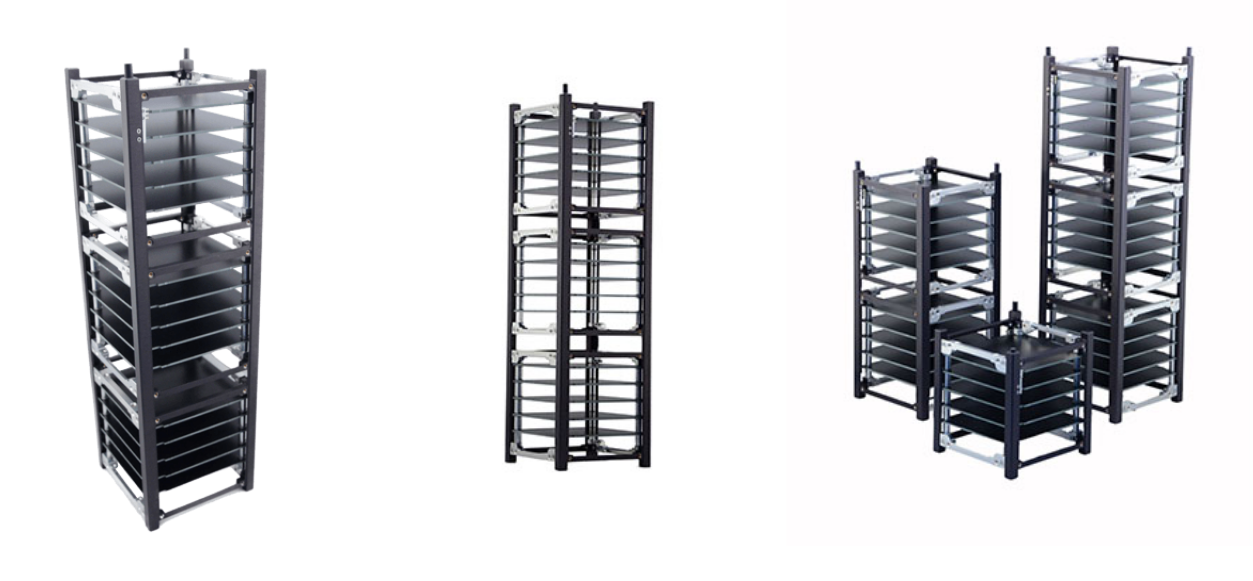
\includegraphics[width=\textwidth]{img/structures_3u.png}
	\caption{Different pictures of the 3U structure}
	\label{fig:structures_3u}
\end{figure}

Furthermore, this structure is one of the cheapest ones, it fulfills the size
standards and its weight is low enough to introduce the required subsystems for
the mission. Moreover, its origin, the ISIS company, ensures the demanded
qualification and acceptance testing. This testing includes functional, vibration,
mechanical shock, thermal cycling and thermal vacuum. In addition, the design of
the structure allows the accessibility of all the flight avionics, even after
the final integration.\\

Then, having chosen the 3U structure, the subsystems must be organised into this
structure. It must taken into account that the CubeSat is always pointing to the
Earth’s surface, Unit 1 points to the deep space and Unit 3 points to the Earth.
Having the size of each subsystem, they have been integrated in the order below.\\

\paragraph{UNIT 1}
The internal part of the unit only comprises the propulsion system, which is the subsystem which requires more volume.\\
On the external part, the solar panels are located there, attached to the final edges of the CubeSat. They will be pointing to the deep space in order to receive the maximum possible solar radiation.\\
Moreover, forming an angle of around \SI{45}{\degree} with the plane of the
deployed solar panels, there will be the four antennas in charge of the
inter-satellite communications.\\

\paragraph{UNIT 2}
This intermediate unit has the function of allocating most of the little subsystems.
It comprises the Electrical Power System, whose energy is supplied from the solar
panels, the Thermal Control System, the Attitude Determination \& Control System
and the Command \& Data Handling with the On-Board Computer.\\
These are many subsystems but they do not take up so much of the unit size. The
EPS and the THC would be allocated in one single board due to their simplicity
and the ADCS takes up a 30\% of the total size of the unit. Finally, as the
CDH is practically part of the payload due to the objective of the mission,
part of it will be allocated in this unit.\\

\paragraph{UNIT 3}
This unit is the one that characterizes the mission. It allocates all the
Communication system together with the rest of the CDH system.\\
At launch phase, the deployable helicoidal antenna, which takes up the
35\% of the whole unit, is allocated inside it. Then, when the CubeSat starts
orbiting, it is deployed and points towards the Earth’s surface. The rest of the
unit is fulfilled with the rest of the required Communications system, which is
the main payload to perform the mission.\\

The overall design of the cubesat can be seen in figure \ref{fig:cubesat_structure}

\begin{figure}[h!]
	\centering
	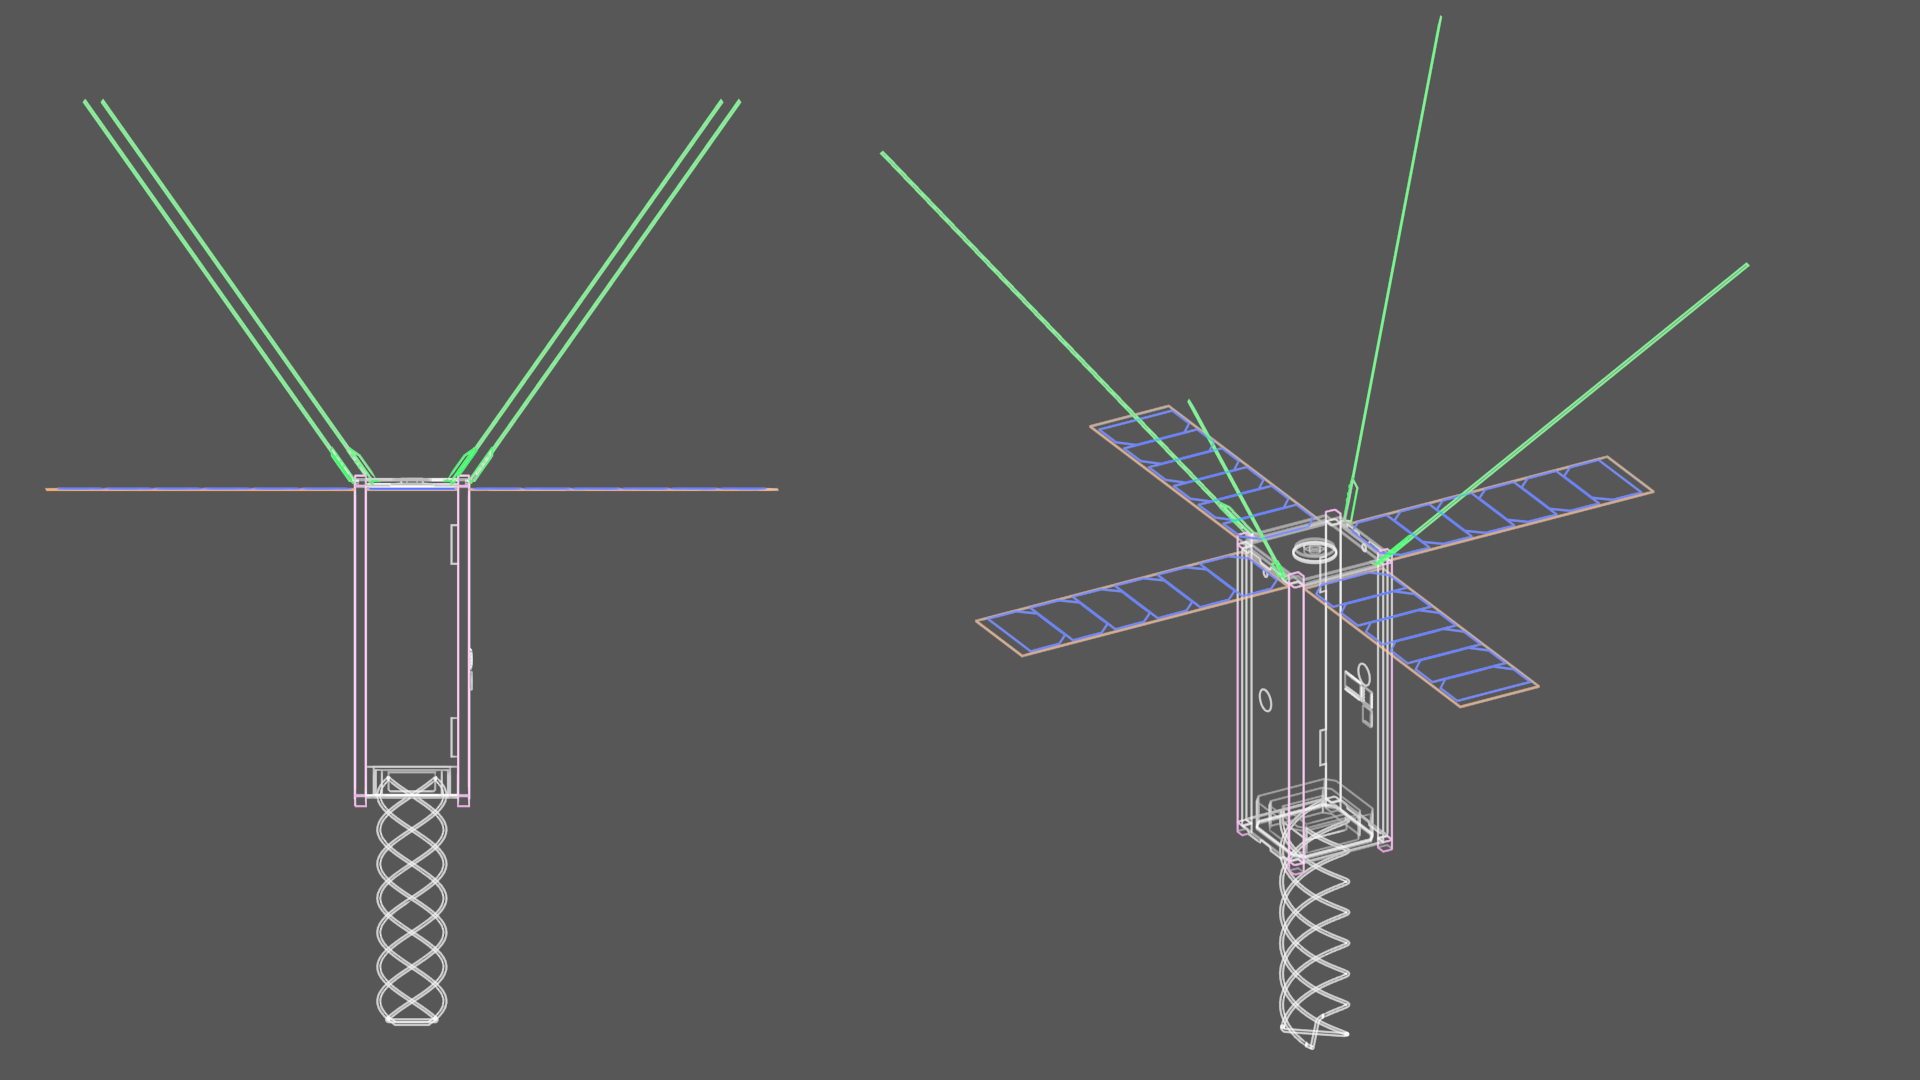
\includegraphics[width=\textwidth]{img/Blueprint_grey.png}
	\caption[Overall satellite structure]{Side and 3d views of the overall satellite structure}
	\label{fig:cubesat_structure}
\end{figure}
